\documentclass[11pt]{beamer}
\usetheme{Warsaw}
\usepackage[utf8]{inputenc}
\usepackage[spanish]{babel}
\usepackage{amsmath,amsthm,amssymb} %modos matemáticos y  simbolos
\usepackage{latexsym,amsfonts} %simbolos matematicos
\usepackage{graphicx}
\usepackage{physics} %Simbolos fisicos
\usepackage{array} %mejores formatos de tabla
\usepackage{tabulary}
\usepackage{multirow} %ocupar varias filas en una tabla
\usepackage{fancybox} %recuadros talegas
\usepackage{float} %ubicar graficas
\usepackage{color}
\usepackage{comment}
\usepackage{stackrel}
\usepackage{calligra}
\usepackage{lipsum} % texto de relleno
\usepackage{cite}
\author{Diego Sarceño}
\title{Lenguajes Regulares}
%\setbeamercovered{transparent} 
%\setbeamertemplate{navigation symbols}{} 
%\logo{} 
%\institute{} 
\date{\today} 
%\subject{} 
\begin{document}

\begin{frame}
\titlepage
\end{frame}

%\begin{frame}
%\tableofcontents
%\end{frame}

\frame{
	\frametitle{Cerradura bajo la Concatenación}
	La clase de lenguajes regulares es cerrada bajo la operación de concatenación. (Lenguajes bajo el mismo alfabeto.)
}

\frame{
	\frametitle{Idea de la Demostración}
	Dados dos lenguajes $A_1$ y $A_2$, se define la concatenación como
		$$
			A_1 \circ A_2 = A_1 A_2 = \{ xy | x\in A_1 \, \land \, y\in A_2 \} .
		$$
	Con esta definición en mente, se trabajará parecido al caso de la union, con la salvedad de que en vez de ser AFDs serán AFNDs. Se tomarán $N_1$ y $N_2$ AFNDs que reconozcan a $A_1$ y $A_2$. Se construirá un AFND que acepte estados como si fueran partidos en dos pedazos, en concreto, pedazos que acepte $N_1$ y el otro pedazo lo acepte $N_2$. \\
	
		
}

\frame{
	\frametitle{Visualización de la Idea}
	Ya con esta idea, lo que vamos a hacer (visualmente) es:
	\begin{figure}[H]
		\centering
		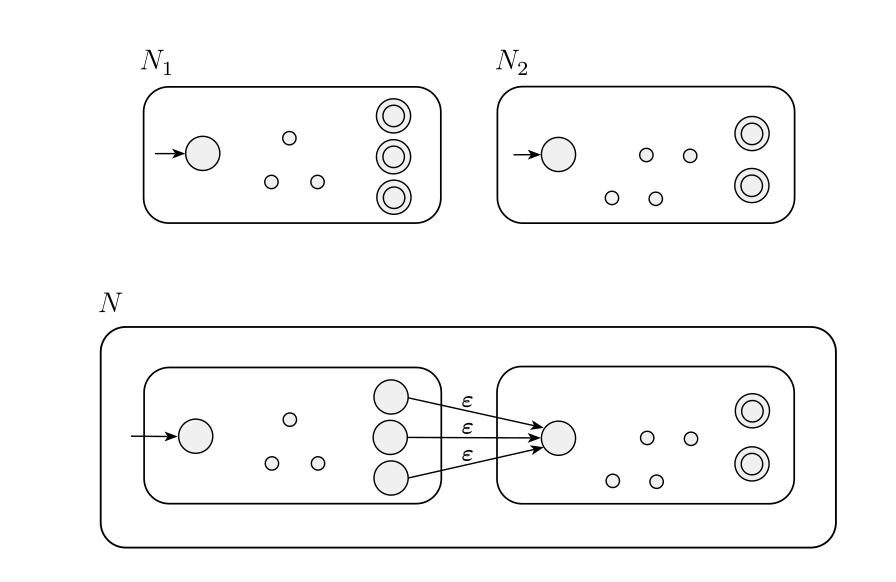
\includegraphics[scale=0.3]{./img/concatenacion.png}
	\end{figure}
}


\frame{
	\frametitle{Desarrollo}
	\onslide<1->{
	Ya con esto, se definen los AFNDs $N_1 = ( Q_1,\Sigma ,\delta _1 ,q_1 ,F_1 )$ y $N_2 = ( Q_2 ,\Sigma , \delta _2, q_2 ,F_2 )$. Ahora construímos $N$ como $N = ( Q,\Sigma ,\delta ,q_1 ,F_2 )$:
	}
	\begin{enumerate}
		\item \onslide<2->{ $Q = Q_1 \cup Q_2$, dado que queremos tener todos los estados de ambos autómatas.}
		\item \onslide<3->{ El alfabeto no cambia. }
		\item \onslide<4->{ La función de transición se vuelve una función por casos, tomando $x\in \Sigma$ y $q \in Q$
			$$ \delta (q,x) = 
				\left\{\begin{array}{rl}
					\delta _1 (q,x) & q\in Q_1 \quad \text{y} \quad q\notin F_1 \\
					\delta _1 (q,x) & x\neq \varepsilon \\
					\delta _2 (q,x) \cup \{ q_2 \} & q \in F_1 \quad \text{y} \quad x = \varepsilon \\
					\delta _2 (q,x) & q\in Q_2 \\
				\end{array}\right.
			$$}
		\item \onslide<5->{ El estado inicial es el de $N_1$ y los estados de aceptación son los de $N_2$.}
	\end{enumerate}
}

\frame{
	\frametitle{$N$ Acepta toda cadena de $A_1 A_2$}
}

\frame{
	\frametitle{Cerradura bajo la Clausura de Kleene}
	La clase de lenguajes regulares es cerrada bajo la Clausura de Kleene.
}

\frame{
	\frametitle{Idea de la Demostración}
	Dado el lenguaje $A$, la clausura de Kleene se define como
		$$
			A^* = \{ x_0 x_1 \cdots x_n \, | \, n \geq 0, \quad x_i \in A \} ,		
		$$
	Para esta prueba, se agregará un nuevo estado inicial (que también será de aceptación), puesto que es necesario aceptar la cadena vacía; además, el conjunto de estados de aceptación debe estar conectado con el estado inicial del autómata original. Esto será más claro en la siguiente diapositiva.
}

\frame{
	\frametitle{Visualización de la Idea}
	\begin{figure}[H]
		\centering
		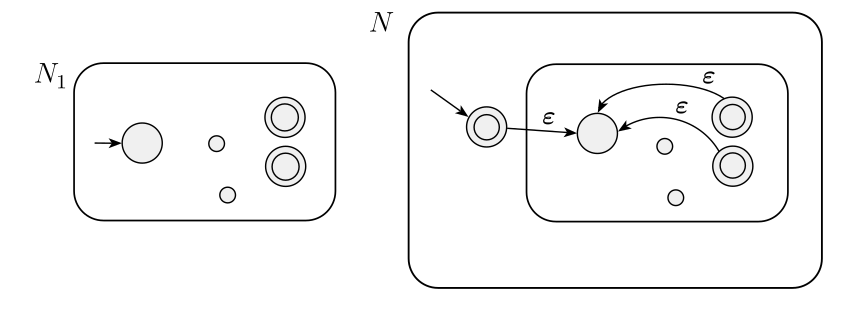
\includegraphics[scale=0.3]{./img/kleene.png}
	\end{figure}
}

\frame{
	\frametitle{Desarrollo}
	\onslide<1->{ Tomando $N_1 = ( Q_1 ,\Sigma ,\delta _1 , q_1 ,F_1 )$, y se construye $N = ( Q,\Sigma ,\delta ,q_o ,F )$, donde}
	\begin{enumerate}
		\item \onslide<2->{ $Q\cup \{ q_o \}$ }
		\item \onslide<3->{ Tomando $q\in Q$ y $a\in \Sigma _\varepsilon$
				$$ \delta (q,x) = 
					\left\{\begin{array}{rl}
						\delta _1 (q,x) & q\in Q_1 , \quad q\notin F \\
						\delta _1 (q,x) & q\in F, \quad a\neq \varepsilon \\
						\delta _1 (q,x) \cup \{ q_1 \} & a = \varepsilon \\
						\{ q_1 \} & q = q_o \quad a = \varepsilon \\
						\emptyset & q = q_o \quad a \neq \varepsilon
					\end{array}\right.
				$$
		}
		\item \onslide<4->{ Estado inicial $q_o$ }
		\item \onslide<5->{ $F = F_1 \cup \{ q_o \}$ }
	\end{enumerate}
		
}















\end{document}